\documentclass[aspectratio=169]{beamer}
\mode<presentation> {
\usetheme{default}
\usecolortheme{dolphin}
}
\usepackage{algorithm,algorithmic}
\usepackage{caption}
\usepackage{multirow}
\usepackage{threeparttable}
\usepackage{graphicx}
\usepackage{parskip}
\usepackage{float}
\usepackage{alphabeta}
\usepackage{multirow,array}
\usepackage{subfig}
\usepackage{amsmath}
\usepackage{amssymb}
\usepackage{mathabx}
\usepackage{caption}
\usepackage{pifont} 
\usepackage{booktabs,tabularx}
\usepackage{tikz}
\usetikzlibrary{shapes,arrows}
\usepackage[table]{xcolor}
\newcolumntype{Y}{>{\raggedright\arraybackslash}X}

\usepackage{tikz}
\usetikzlibrary{arrows.meta,positioning,calc,fit,backgrounds,decorations.pathreplacing, shapes.geometric}
\graphicspath{{figures/}}
\usetikzlibrary{matrix,chains,positioning,decorations.pathreplacing,arrows}

% TikZ Styles - Adjusted font sizes for clarity since bold is removed
\tikzset{
  >=Stealth,
  st/.style={circle,draw,inner sep=0pt,minimum size=6mm, fill=white}, 
  action/.style={circle,fill=black,inner sep=0pt,minimum size=2mm},
  tr/.style={-Stealth, line width=0.8pt},
  lbl/.style={font=\footnotesize},
  block/.style={rectangle, draw, fill=blue!10, rounded corners, minimum height=2em}
}

\newcommand{\E}{\mathbb{E}}
\newcommand{\R}{\mathbb{R}}
\newcommand{\1}{\mathbf{1}}
\newcommand{\loss}{\mathcal{L}}
\newcommand{\X}{\mathcal{X}}
\newcommand{\Y}{\mathcal{Y}}
\newcommand{\D}{\mathcal{D}}
\newcommand{\thetavec}{\boldsymbol{\theta}}
\DeclareMathOperator*{\argmax}{arg\,max}
\DeclareMathOperator*{\argmin}{arg\,min}
\setbeamertemplate{caption}[numbered]
\setbeamertemplate{navigation symbols}{}
\setbeamertemplate{footline}[frame number]

\title{Reinforcement Learning}

\author{Yasuyuki Sawada, Yaolang Zhong}
\institute{University of Tokyo\\
  \small \texttt{\href{mailto:yaolang.zhong@e.u-tokyo.ac.jp}{yaolang.zhong@e.u-tokyo.ac.jp}}}
\date{}

\begin{document}

\begin{frame}
\titlepage  
\end{frame}



\begin{frame}{Recap: Motivation for Machine Learning}
  \begin{itemize}
      \item Dynamic programming faces the curse of dimensionality
      \begin{itemize}
          \item Parameterization problem
          \begin{itemize}
              \item Classical functional forms (linear, polynomials, splines)
              \item Number of basis terms grows rapidly with state dimension
              \item Strong restrictions and poor capture of interactions
          \end{itemize}
          \item Grid / data problem
          \begin{itemize}
              \item Grid-based DP requires $N^d$ state points
              \item Computation and memory grow exponentially
              \item Sparse grids mitigate but do not eliminate the problem
          \end{itemize}
      \end{itemize}
  \end{itemize}
  \end{frame}

  \begin{frame}{How Machine Learning Addresses the Curse of Dimensionality}
    \begin{itemize}
        \item Machine learning relaxes both constraints
        \begin{itemize}
            \item \textcolor{blue}{Neural networks for parameterization}
            \begin{itemize}
                \item \textcolor{blue}{Flexible, high-dimensional function approximation}
                \item \textcolor{blue}{Captures nonlinearities and interactions}
            \end{itemize}
            \item Stochastic simulation for data collection
            \begin{itemize}
                \item Learn from simulated trajectories, not full grids
                \item Scales to high-dimensional state spaces
            \end{itemize}
        \end{itemize}
    \end{itemize}
    \end{frame}


    \begin{frame}{Overview}
      \small
      \begin{enumerate}
          \item Network Architecture
          \begin{itemize}
              \item Actor: policy network $\sigma(s;\theta)$ maps states to actions
              \item Critic: value network $Q(s,a;\phi)$ evaluates state--action pairs
          \end{itemize}
          \item Forward Pass
          \begin{itemize}
              \item Batch of states $S \in \mathbb{R}^{N \times D_S}$
              \item Actor produces actions; critic produces value estimates
          \end{itemize}
          \item Objective Functions
          \begin{itemize}
              \item Actor: maximize expected return via policy gradient
              \item Critic: minimize Bellman residual (temporal difference error)
          \end{itemize}
          \item Backward Pass and Parameter Updates
          \begin{itemize}
              \item Compute gradients $\nabla_\theta \mathcal{L}_\theta$ and $\nabla_\phi \mathcal{L}_\phi$
              \item Update parameters via gradient descent
          \end{itemize}
          \item Implementation Caveats
          \begin{itemize}
              \item Target networks for training stability
              \item Gradient detachment to separate actor and critic updates
          \end{itemize}
      \end{enumerate}
      \end{frame}




\begin{frame}{Actor--Critic Methods: Introduction}
  \begin{itemize}
      \item Actor--critic methods are a general framework for reinforcement learning (RL) problem
      \item Particularly suited for Large or continuous state spaces and action spaces
      \item The framework decomposes learning into policy learning (actor) and value learning (critic)
      \begin{itemize}
        \item Actor: a parameterized policy $\sigma(a \mid s; \theta)$ that selects actions
        \item Critic: a parameterized value function $Q(s,a; \phi)$ that provides an evaluation signal guiding policy improvement
        \item The notation $\sigma(a \mid s; \theta)$ denotes a (possibly stochastic) policy: the probability of choosing action $a$ in state $s$ given parameters $\theta$; deterministic policies are a special case that assign probability one to a single action (often written simply as $\sigma(s)$)
      \end{itemize}
  \end{itemize}
  \end{frame}

% -------------------------------------------------
% Actor-Critic Network Architecture Diagram
% -------------------------------------------------
\begin{frame}{Actor Network Architecture}
\centering
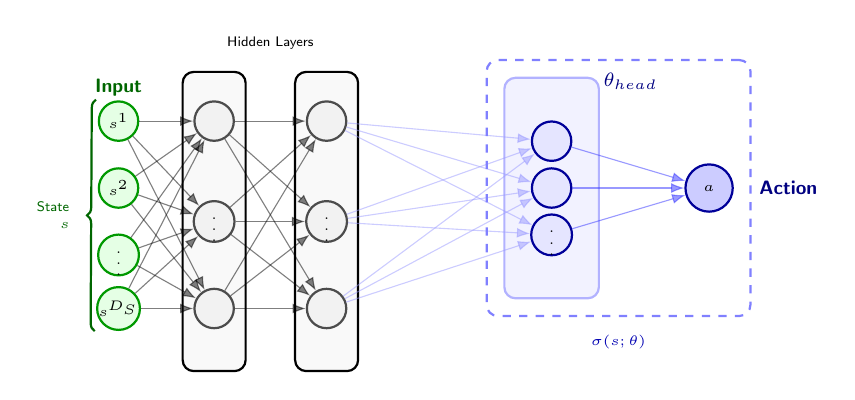
\begin{tikzpicture}[x=1.0cm, y=0.85cm, 
    % Neural network styles for this figure
    neuron/.style={circle, draw, thick, minimum size=0.5cm, inner sep=0pt, fill=white, font=\tiny},
    input neuron/.style={neuron, fill=green!10, draw=green!60!black},
    hidden neuron/.style={neuron, fill=gray!10, draw=gray!60!black},
    actor neuron/.style={neuron, fill=blue!10, draw=blue!60!black},
    connect/.style={-Latex, thin, opacity=0.5},
    layer box/.style={rectangle, draw, thick, rounded corners, inner sep=5pt, align=center, fill=gray!5},
    label text/.style={font=\sffamily\tiny},
    section label/.style={font=\sffamily\bfseries\scriptsize}
]

% --- Input Layer (State s) ---
\node[section label, green!40!black] at (0, 1.5) {Input};
\foreach \i in {1,0} {
    \node[input neuron] (I\i) at (0, \i) {$s^{\pgfmathparse{int(2-\i)}\pgfmathresult}$};
}
\node[input neuron] (Idots) at (0, -1) {$\vdots$};
\node[input neuron] (In) at (0, -1.8) {$s^{D_S}$};

% Group inputs with a brace
\draw[decorate, decoration={brace, amplitude=3pt, mirror}, thick, green!40!black] 
    ($(I1.north west)+(-0.1,0.1)$) -- ($(In.south west)+(-0.1,-0.1)$) 
    node[midway, left=0.2cm, align=right, label text] {State\\$s$};

% --- Hidden Layer 1 ---
\node[layer box, right=0.8cm of $(I0)!0.5!(Idots)$, minimum height=3.8cm, minimum width=0.8cm] (hiddenBlock1) {};
\node[hidden neuron] (H1a) at (hiddenBlock1.center |- I1) {};
\node[hidden neuron] (H1dots) at (hiddenBlock1.center) {$\vdots$};
\node[hidden neuron] (H1n) at (hiddenBlock1.center |- In) {};

% --- Hidden Layer 2 ---
\node[layer box, right=0.6cm of hiddenBlock1, minimum height=3.8cm, minimum width=0.8cm] (hiddenBlock2) {};
\node[hidden neuron] (H2a) at (hiddenBlock2.center |- I1) {};
\node[hidden neuron] (H2dots) at (hiddenBlock2.center) {$\vdots$};
\node[hidden neuron] (H2n) at (hiddenBlock2.center |- In) {};

\node[label text, above=0.15cm of $(hiddenBlock1.north)!0.5!(hiddenBlock2.north)$] {Hidden Layers};

% Connect Inputs to Hidden Layer 1
\foreach \i in {I1, I0, Idots, In} {
    \foreach \h in {H1a, H1dots, H1n} {
        \draw[connect] (\i) -- (\h);
    }
}

% Connect Hidden Layer 1 to Hidden Layer 2
\foreach \ha in {H1a, H1dots, H1n} {
    \foreach \hb in {H2a, H2dots, H2n} {
        \draw[connect] (\ha) -- (\hb);
    }
}

% --- Actor Head (Policy) ---
\node[layer box, minimum height=2.8cm, minimum width=1.2cm, fill=blue!5, draw=blue!30] (actorBlock) at (5.5, 0) {};
\node[section label, blue!50!black] at (6.5, 1.6) {$\theta_{head}$};
\node[actor neuron] (AH1) at (5.5, 0.7) {};
\node[actor neuron] (AH2) at (5.5, 0) {};
\node[actor neuron] (AHdots) at (5.5, -0.7) {$\vdots$};

% Actor Output Layer (single action output)
\node[actor neuron, fill=blue!20, minimum size=0.6cm] (Aout) at (7.5, 0) {$a$};

% Connections from hidden to actor
\foreach \h in {H2a, H2dots, H2n} { \foreach \ah in {AH1, AH2, AHdots} { \draw[connect, blue!40] (\h) -- (\ah); } }
\foreach \ah in {AH1, AH2, AHdots} { \draw[connect, blue!80] (\ah) -- (Aout); }

\node[right=0.2cm of Aout, section label, blue!50!black] {Action};

% --- Dashed box for Actor ---
\node[draw=blue!50, thick, dashed, rounded corners, fit=(actorBlock) (Aout), inner sep=6pt] (actorGroup) {};
\node[below=0.1cm of actorGroup, blue!70!black, font=\bfseries\tiny] {$\sigma(s;\theta)$};

\end{tikzpicture}
\end{frame}

% -------------------------------------------------
% Critic Network Architecture Diagram
% -------------------------------------------------
\begin{frame}{Critic Network Architecture}
\centering
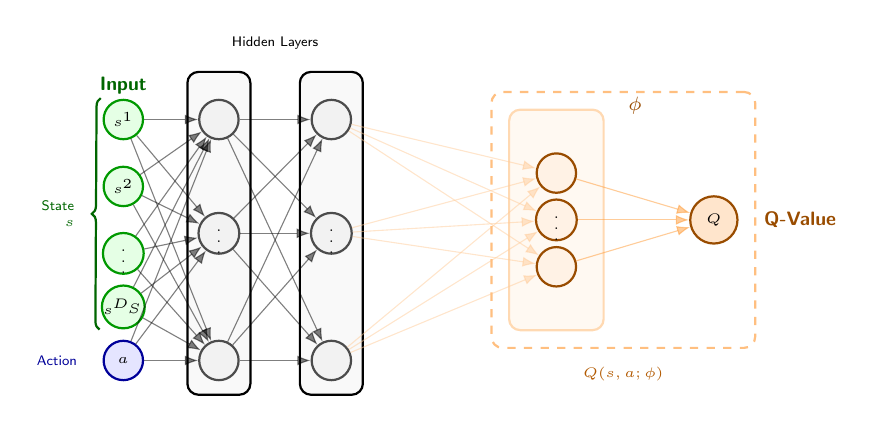
\begin{tikzpicture}[x=1.0cm, y=0.85cm, 
    % Neural network styles for this figure
    neuron/.style={circle, draw, thick, minimum size=0.5cm, inner sep=0pt, fill=white, font=\tiny},
    input neuron/.style={neuron, fill=green!10, draw=green!60!black},
    action neuron/.style={neuron, fill=blue!10, draw=blue!60!black},
    hidden neuron/.style={neuron, fill=gray!10, draw=gray!60!black},
    q neuron/.style={neuron, fill=orange!10, draw=orange!60!black},
    connect/.style={-Latex, thin, opacity=0.5},
    layer box/.style={rectangle, draw, thick, rounded corners, inner sep=5pt, align=center, fill=gray!5},
    label text/.style={font=\sffamily\tiny},
    section label/.style={font=\sffamily\bfseries\scriptsize}
]

% --- Input Layer (State s and Action a) ---
\node[section label, green!40!black] at (0, 1.5) {Input};
\foreach \i in {1,0} {
    \node[input neuron] (I\i) at (0, \i) {$s^{\pgfmathparse{int(2-\i)}\pgfmathresult}$};
}
\node[input neuron] (Idots) at (0, -1) {$\vdots$};
\node[input neuron] (In) at (0, -1.8) {$s^{D_S}$};
\node[action neuron] (Ia) at (0, -2.6) {$a$};

% Group state inputs with a brace
\draw[decorate, decoration={brace, amplitude=3pt, mirror}, thick, green!40!black] 
    ($(I1.north west)+(-0.1,0.1)$) -- ($(In.south west)+(-0.1,-0.1)$) 
    node[midway, left=0.2cm, align=right, label text] {State\\$s$};

% Label for action
\node[left=0.2cm of Ia, label text, blue!60!black] {Action};

% --- Hidden Layer 1 ---
\node[layer box, right=0.8cm of $(I0)!0.7!(Idots)$, minimum height=4.1cm, minimum width=0.8cm] (hiddenBlock1) {};
\node[hidden neuron] (H1a) at (hiddenBlock1.center |- I1) {};
\node[hidden neuron] (H1dots) at (hiddenBlock1.center) {$\vdots$};
\node[hidden neuron] (H1n) at (hiddenBlock1.center |- Ia) {};

% --- Hidden Layer 2 ---
\node[layer box, right=0.6cm of hiddenBlock1, minimum height=4.1cm, minimum width=0.8cm] (hiddenBlock2) {};
\node[hidden neuron] (H2a) at (hiddenBlock2.center |- I1) {};
\node[hidden neuron] (H2dots) at (hiddenBlock2.center) {$\vdots$};
\node[hidden neuron] (H2n) at (hiddenBlock2.center |- Ia) {};

\node[label text, above=0.15cm of $(hiddenBlock1.north)!0.5!(hiddenBlock2.north)$] {Hidden Layers};

% Connect Inputs to Hidden Layer 1
\foreach \i in {I1, I0, Idots, In, Ia} {
    \foreach \h in {H1a, H1dots, H1n} {
        \draw[connect] (\i) -- (\h);
    }
}

% Connect Hidden Layer 1 to Hidden Layer 2
\foreach \ha in {H1a, H1dots, H1n} {
    \foreach \hb in {H2a, H2dots, H2n} {
        \draw[connect] (\ha) -- (\hb);
    }
}

% --- Q Head ---
\node[layer box, minimum height=2.8cm, minimum width=1.2cm, fill=orange!5, draw=orange!30] (qBlock) at (5.5, -0.5) {};
\node[section label, orange!60!black] at (6.5, 1.2) {$\phi$};
\node[q neuron] (QH1) at (5.5, 0.2) {};
\node[q neuron] (QHdots) at (5.5, -0.5) {$\vdots$};
\node[q neuron] (QHn) at (5.5, -1.2) {};

% Q Output
\node[q neuron, fill=orange!20, minimum size=0.6cm] (Qout) at (7.5, -0.5) {$Q$};

% Connections from hidden to Q head
\foreach \h in {H2a, H2dots, H2n} { \foreach \qh in {QH1, QHdots, QHn} { \draw[connect, orange!40] (\h) -- (\qh); } }
\foreach \qh in {QH1, QHdots, QHn} { \draw[connect, orange!80] (\qh) -- (Qout); }

\node[right=0.2cm of Qout, section label, orange!60!black] {Q-Value};

% --- Dashed box for Q network ---
\node[draw=orange!50, thick, dashed, rounded corners, fit=(qBlock) (Qout), inner sep=6pt] (qGroup) {};
\node[below=0.1cm of qGroup, orange!70!black, font=\bfseries\tiny] {$Q(s,a;\phi)$};

\end{tikzpicture}
\end{frame}


\begin{frame}{Forward Pass}
\small
  \begin{itemize}
      \item Suppose a batch of states available: $\{ s_i \}_{i=1}^N$ where $s_i \in \mathbb{R}^{D_S}$, stacked as $S \in \mathbb{R}^{N \times D_S}$
      \item Two neural networks:
      \begin{itemize}
          \item Actor: $\sigma(s;\theta)$
          \item Critic: $Q(s,a;\phi)$
      \end{itemize}
      \item Forward Pass:
        \begin{alignat*}{3}
          S &\in \mathbb{R}^{N \times D_S} \quad&& \xrightarrow{\;\;\theta\;\;} \quad& A &\in \mathbb{R}^{N \times D_A}\\
          (S,A) &\in \mathbb{R}^{N \times (D_S+D_A)} \quad&& \xrightarrow{\;\;\phi\;\;} \quad& Q &\in \mathbb{R}^{N}
        \end{alignat*}

      \item Training vs.\ evaluation:
      \begin{itemize}
          \item In \emph{training mode}, the forward pass constructs a computational graph and records gradients with respect to the network parameters
          \item In \emph{evaluation mode}, the same forward mappings are applied, but no gradients are recorded
      \end{itemize}

  \end{itemize}
\end{frame}






\begin{frame}{Backward Propagation: Intuition}
  \small
  \begin{itemize}
      \item In training mode, once a scalar loss $\mathcal{L}$ is defined, the gradient $\nabla_\theta \mathcal{L}$ is computed automatically by back-propagation in any ML package.
      \item Backpropagation applies the chain rule through the computational graph constructed in the forward pass
  

      \item The actor and critic would be updated via gradient descent (although in practice, more stochastic methods are used) as:
      $$
      \theta \leftarrow \theta - \alpha_\theta \nabla_\theta \mathcal{L}_\theta
      $$
      $$
      \phi \leftarrow \phi - \alpha_\phi \nabla_\phi \mathcal{L}_\phi
      $$

      \item The question is how to construct the loss function $\mathcal{L}$ for the actor and critic.
  
  \end{itemize}
  \end{frame}

  \begin{frame}{Backward Propagation: Actor Objective (1/2)}
    \small
    \begin{itemize}
        \item The actor aims to maximize expected discounted returns:
        \[
            J(\theta)
            =
            \mathbb{E}_{\tau \sim P_\theta}
            \big[ R(\tau) \big],
            \qquad
            R(\tau) \equiv \sum_{k=0}^{\infty} \gamma^k r_k
        \]
    
        \item The policy gradient can be written as:
        \[
            \nabla_\theta J(\theta)
            =
            \mathbb{E}
            \left[
                \sum_{t=0}^{\infty}
                \nabla_\theta \log \sigma(a_t \mid s_t;\theta)\;
                \gamma^t G_t
            \right],
            \qquad
            G_t \equiv \sum_{k=t}^{\infty} \gamma^{k-t} r_k
        \]
    
        \item Realized returns $G_t$ are noisy and depend on the entire future trajectory
    
        \item For a given policy $\sigma(a \mid s;\theta)$, the state--action value satisfies:
        \[
            Q^\sigma(s_t,a_t)
            =
            \mathbb{E}[\,G_t \mid s_t, a_t\,]
        \]
    \end{itemize}
\end{frame}

\begin{frame}{Backward Propagation: Actor Objective (2/2)}
    \small
    \begin{itemize}
        \item By iterated expectations, replacing $G_t$ with $Q^\sigma(s_t,a_t)$ is exact in expectation:
        \[
            \mathbb{E}\!\left[
            \nabla_\theta \log \sigma(a_t \mid s_t;\theta)\, G_t
            \right]
            =
            \mathbb{E}\!\left[
            \nabla_\theta \log \sigma(a_t \mid s_t;\theta)\, Q^\sigma(s_t,a_t)
            \right]
        \]
    
        \item In practice, the true $Q^\sigma$ is unknown; we use the current critic estimate $Q(s,a;\phi)$
    
        \item Sample-based actor loss (depends on current critic parameters $\phi$):
        \[
            \mathcal{L}_\theta
            =
            -\frac{1}{N}
            \sum_{i=1}^{N}
            \sum_{t=1}^{T_i}
            \log \sigma(a_{i,t} \mid s_{i,t};\theta)\;
            \gamma^t Q(s_{i,t},a_{i,t};\phi)
        \]

        \item The critic $Q(s,a;\phi)$ provides a lower-variance learning signal compared to realized returns
    \end{itemize}
\end{frame}






% 1/4: Likelihood-Ratio Reformulation, with explicit return definition and explanation
\begin{frame}{Policy Gradient Derivation* (1/4: Likelihood-Ratio Reformulation)}
    \small
    \begin{itemize}
        \item Start from the RL objective in integral form:
        \[
            J(\theta)
            =
            \mathbb{E}_{\tau \sim P_\theta}[R(\tau)]
            =
            \int R(\tau)\, P_\theta(\tau)\, d\tau, \quad \text{where} \quad R(\tau) \equiv \sum_{k=0}^{\infty} \gamma^k r_k
        \]

        \item Differentiate under the integral sign:
        \[
            \nabla_\theta J(\theta)
            =
            \int R(\tau)\, \nabla_\theta P_\theta(\tau)\, d\tau
        \]
        \item Use $\nabla_\theta P_\theta(\tau) = P_\theta(\tau) \nabla_\theta \log P_\theta(\tau)$:
        \[
            \nabla_\theta J(\theta)
            =
            \int R(\tau)\, P_\theta(\tau)\, \nabla_\theta \log P_\theta(\tau)\, d\tau
        \]
        \item Convert to expectation:
        \[
            \nabla_\theta J(\theta)
            =
            \mathbb{E}_{\tau \sim P_\theta}
            \left[
                \nabla_\theta \log P_\theta(\tau)\; R(\tau)
            \right]
        \]
    \end{itemize}
    This is the likelihood-ratio (score-function) trick.
\end{frame}
    
    % -----------------------------------------------
    % Trajectory likelihood (*)
    % -----------------------------------------------
\begin{frame}{Policy Gradient Derivation* (2/4: Trajectory Likelihood Factorization)}
\small
\begin{itemize}
    \item Trajectory density factorizes as
    \[
        P_\theta(\tau)
        =
        p(s_0)
        \prod_{t=0}^{\infty}
        \sigma(a_t \mid s_t;\theta)
        \, P(s_{t+1} \mid s_t,a_t)
    \]
    \item Only the policy depends on $\theta$, hence
    \[
        \nabla_\theta \log P_\theta(\tau)
        =
        \sum_{t=0}^{\infty}
        \nabla_\theta \log \sigma(a_t \mid s_t;\theta)
    \]
\end{itemize}

Environment transition terms drop out of the gradient.
\end{frame}
    
% -----------------------------------------------
% Policy Gradient Theorem (*): clean substitution
% -----------------------------------------------
\begin{frame}{Policy Gradient Derivation* (3/4: Causality)}
    \small
    \begin{itemize}
        \item Substitute the log-policy sum and expand $R(\tau)$:
        \[
            \nabla_\theta J(\theta)
            =
            \mathbb{E}_{\tau \sim P_\theta}
            \left[
                \left(
                \sum_{t=0}^{\infty} \nabla_\theta \log \sigma(a_t \mid s_t;\theta)
                \right)
                \left(
                \sum_{k=0}^{\infty} \gamma^k r_k
                \right)
            \right]
        \]
        \item Swap the order of summation:
        \[
            \nabla_\theta J(\theta)
            =
            \mathbb{E}_{\tau \sim P_\theta}
            \left[
                \sum_{t=0}^{\infty}
                \sum_{k=0}^{\infty}
                \nabla_\theta \log \sigma(a_t \mid s_t;\theta)\;
                \gamma^k r_k
            \right]
        \]
        \item \textbf{Causality:} For each $t$, terms with $k < t$ have zero expectation, since rewards before $t$ do not depend on $a_t$. Therefore, restrict inner sum to $k \geq t$:
        \[
            =
            \mathbb{E}
            \left[
                \sum_{t=0}^{\infty}
                \nabla_\theta \log \sigma(a_t \mid s_t;\theta)\;
                \sum_{k=t}^{\infty} \gamma^k r_k
            \right]
        \]
        \item Define the return from $t$: $G_t \equiv \sum_{k=t}^{\infty} \gamma^{k-t} r_k$, so $\sum_{k=t}^{\infty} \gamma^k r_k = \gamma^t G_t$
    \end{itemize}
\end{frame}
    
    
    % -----------------------------------------------
    % Actor objective (*): define $G_t$ cleanly
    % -----------------------------------------------
\begin{frame}{Policy Gradient Derivation* (4/4: Surrogate Objective)}
    \small
    \begin{itemize}
        \item Substitute $G_t$ and collect terms:
        \[
            \nabla_\theta J(\theta)
            =
            \mathbb{E}
            \left[
                \sum_{t=0}^{\infty}
                \nabla_\theta \log \sigma(a_t \mid s_t;\theta)\;
                \gamma^t G_t
            \right]
        \]
        \item \textbf{Surrogate objective:}
        \[
            \max_\theta\;
            \mathbb{E}
            \left[
                \sum_{t=0}^{\infty}
                \log \sigma(a_t \mid s_t;\theta)\;
                \gamma^t G_t
            \right]
        \]
        \item This surrogate is constructed so that its gradient with respect to $\theta$ equals the true policy gradient $\nabla_\theta J(\theta)$.
        \item We maximize the surrogate because it is differentiable from sampled data and enables gradient-based optimization of the policy.
        \item Sample-based approximation:
        \[
            \widehat{J}(\theta)
            =
            \frac{1}{N}
            \sum_{i=1}^{N}
            \sum_{t=1}^{T_i}
            \log \sigma(a_{i,t} \mid s_{i,t};\theta)\;
            \gamma^t G_{i,t}
        \]
    \end{itemize}
\end{frame}




\begin{frame}{Backward Propagation: Critic Objective}
    \small
    \begin{itemize}
        \item The critic aims to approximate the state--action value function $Q^\sigma(s,a)$
    
        \item The true $Q^\sigma$ satisfies the Bellman equation:
        \[
            Q^\sigma(s_t,a_t)
            =
            r_t + \gamma \, \mathbb{E}_{s_{t+1}}
            \big[ Q^\sigma(s_{t+1}, a_{t+1}) \big]
        \]
        \item Sample-based critic loss (mean squared Bellman error):
        \[
            \mathcal{L}_\phi
            =
            \frac{1}{N}
            \sum_{i=1}^{N}
            \big( Q(s_i,a_i;\phi) - (r_i + \gamma \mathbb{E}_{s_{i+1}} [Q(s_{i+1}, a_{i+1};\phi)]) \big)^2
        \]
    \end{itemize}
\end{frame}






% -------------------------------------------------
% Implementation Caveat 1: Target Networks
% -------------------------------------------------
\begin{frame}{Implementation Caveat 1: Target Networks}
    \small
    \begin{itemize}
        \item Problem: The critic loss depends on its own predictions
        \[
            \mathcal{L}_\phi = \frac{1}{N}\sum_{i=1}^{N}
            \big( Q(s_i,a_i;\phi) - \underbrace{(r_i + \gamma Q(s_{i+1}, a_{i+1};\phi))}_{\text{target uses same } \phi} \big)^2
        \]
        \item This creates a \emph{moving target} problem $\Rightarrow$ training instability
        
        \item Solution: Use separate \emph{target networks} $\phi_{\text{target}}, \theta_{\text{target}}$
        \[
            y_i = r_i + \gamma Q(s_{i+1}, \sigma(s_{i+1};\theta_{\text{target}}); \phi_{\text{target}})
        \]
        
        \item Target networks are updated slowly:
        \begin{itemize}
            \item Hard update: Copy parameters every $K$ steps
            \item Soft update (Polyak averaging): $\phi_{\text{target}} \leftarrow \tau \phi + (1-\tau)\phi_{\text{target}}$, with $\tau \ll 1$
        \end{itemize}
        
        \item Result: Stable targets $\Rightarrow$ more stable learning
    \end{itemize}
\end{frame}

% -------------------------------------------------
% Implementation Caveat 2: Detaching the Action
% -------------------------------------------------
\begin{frame}{Implementation Caveat 2: Detaching the Action}
  \small
  \begin{columns}[T]
  \begin{column}{0.45\textwidth}
    The \texttt{detach} operation creates a copy of a tensor that is disconnected from the computational graph, blocking gradient propagation.
    \vspace{0.4em}
    \begin{itemize}
        \item The action $a = \sigma(s;\theta)$ is produced by the actor
        \item During critic updates, the action should be treated as fixed input data
        \item Detaching prevents gradients from flowing back to $\theta$
    \end{itemize}
    \vspace{0.4em}
    Implementation:
    \begin{itemize}
        \item \texttt{a\_detached = a.detach()}
        \item Pass \texttt{a\_detached} as input to $Q(s,a;\phi)$
    \end{itemize}
  \end{column}
  \begin{column}{0.52\textwidth}
    \centering
    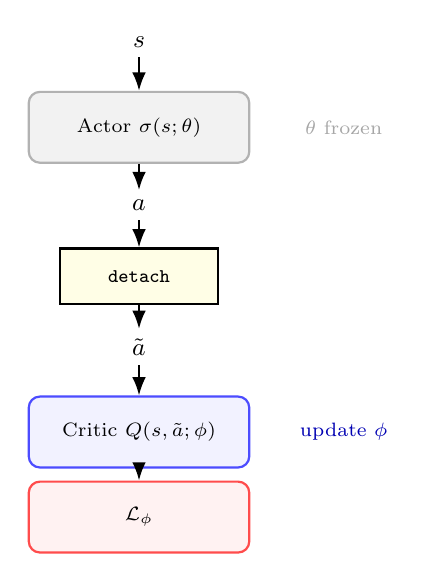
\begin{tikzpicture}[x=1.0cm, y=0.9cm,
        box/.style={draw, thick, rounded corners, minimum width=2.8cm, minimum height=0.9cm, align=center, font=\scriptsize},
        active/.style={box, draw=blue!70, fill=blue!5},
        frozen/.style={box, draw=gray!60, fill=gray!10},
        op/.style={draw, thick, rectangle, minimum width=2.0cm, minimum height=0.7cm, fill=yellow!10, font=\scriptsize},
        loss/.style={box, draw=red!70, fill=red!5},
        arrow/.style={-Latex, thick}
    ]
    \node (s) at (0, 4.2) {\small $s$};
    \node[frozen] (actor) at (0, 3.0) {Actor $\sigma(s;\theta)$};
    \node (a) at (0, 1.9) {\small $a$};
    \node[op] (detach) at (0, 0.9) {\texttt{detach}};
    \node (atilde) at (0, -0.1) {\small $\tilde a$};
    \node[active] (critic) at (0, -1.3) {Critic $Q(s,\tilde a;\phi)$};
    \node[loss] (loss) at (0, -2.5) {$\mathcal L_\phi$};
    \draw[arrow] (s) -- (actor);
    \draw[arrow] (actor) -- (a);
    \draw[arrow] (a) -- (detach);
    \draw[arrow] (detach) -- (atilde);
    \draw[arrow] (atilde) -- (critic);
    \draw[arrow] (critic) -- (loss);
    \node[gray!70, font=\scriptsize, align=center] at (2.6, 3.0) {$\theta$ frozen};
    \node[blue!70!black, font=\scriptsize, align=center] at (2.6, -1.3) {update $\phi$};
    \end{tikzpicture}
  \end{column}
  \end{columns}
  \vspace{0.3em}
  {\footnotesize The critic update optimizes $\phi$ only; the actor is updated separately via policy gradient.}
\end{frame}








\end{document}